\documentclass[border=6pt]{standalone}
\usepackage{tikz}
\usetikzlibrary{arrows.meta,positioning}
\begin{document}
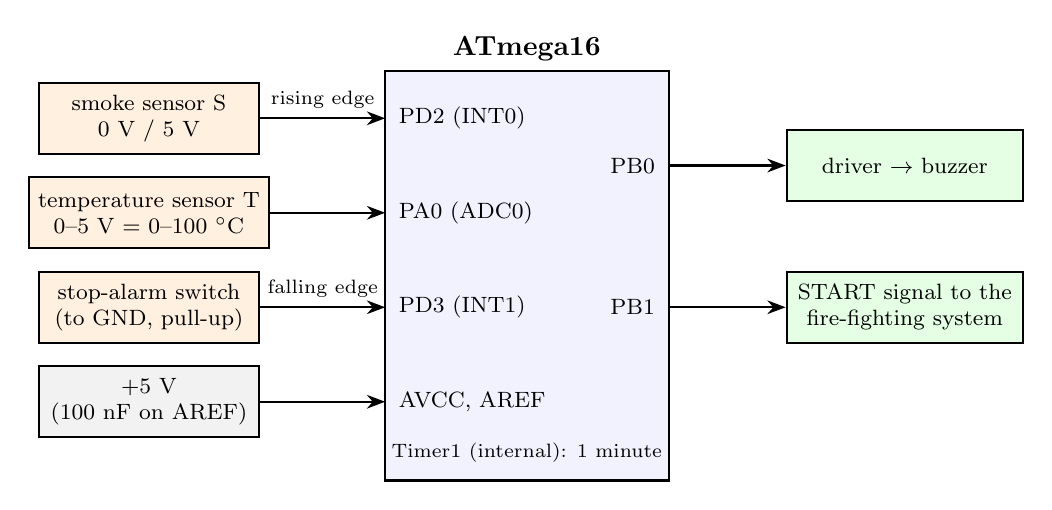
\begin{tikzpicture}[>=Stealth,font=\small,
 dev/.style={draw,thick,fill=orange!12,align=center,font=\footnotesize,minimum width=2.8cm,minimum height=0.9cm},
 outb/.style={draw,thick,fill=green!10,align=center,font=\footnotesize,minimum width=3.0cm,minimum height=0.9cm}]
\draw[thick,fill=blue!5] (0,0) rectangle (3.6,-5.2);
\node[font=\bfseries,anchor=south] at (1.8,0) {ATmega16};
\foreach \y/\t in {-0.6/PD2 (INT0),-1.8/PA0 (ADC0),-3.0/PD3 (INT1),-4.2/{AVCC, AREF}} \node[font=\footnotesize,anchor=west] at (0.05,\y) {\t};
\foreach \y/\t in {-1.2/PB0,-3.0/PB1} \node[font=\footnotesize,anchor=east] at (3.55,\y) {\t};
\node[font=\scriptsize,align=center] at (1.8,-4.85) {Timer1 (internal): 1 minute};
\node[dev] (s) at (-3.0,-0.6) {smoke sensor S\\0 V / 5 V};
\node[dev] (t) at (-3.0,-1.8) {temperature sensor T\\0--5 V = 0--100 $^\circ$C};
\node[dev] (sw) at (-3.0,-3.0) {stop-alarm switch\\(to GND, pull-up)};
\node[dev,fill=gray!10] (p) at (-3.0,-4.2) {+5 V\\(100 nF on AREF)};
\draw[->,thick] (s) -- (0,-0.6) node[pos=0.5,above,font=\scriptsize]{rising edge};
\draw[->,thick] (t) -- (0,-1.8);
\draw[->,thick] (sw) -- (0,-3.0) node[pos=0.5,above,font=\scriptsize]{falling edge};
\draw[->,thick] (p) -- (0,-4.2);
\node[outb] (bz) at (6.6,-1.2) {driver $\to$ buzzer};
\node[outb] (ff) at (6.6,-3.0) {START signal to the\\fire-fighting system};
\draw[->,thick] (3.6,-1.2) -- (bz);
\draw[->,thick] (3.6,-3.0) -- (ff);
\end{tikzpicture}
\end{document}
